\chapter{Branching} % (fold)
\label{cha:branching}

\minitoc

% ============
% = Concepts =
% ============
\section{Branching Concepts} % (fold)
\label{sec:branching_concepts}

\clearpage
\subsubsection{If Statement} % (fold)
\label{sub:if_statement}

The if statement is the most frequently used branching statement. It allows you to selectively run code based on the value of a Boolean expression (the condition). The if statement has an optional \emph{else} branch that is executed when the condition is false.

\begin{figure}[h]
   \centering
   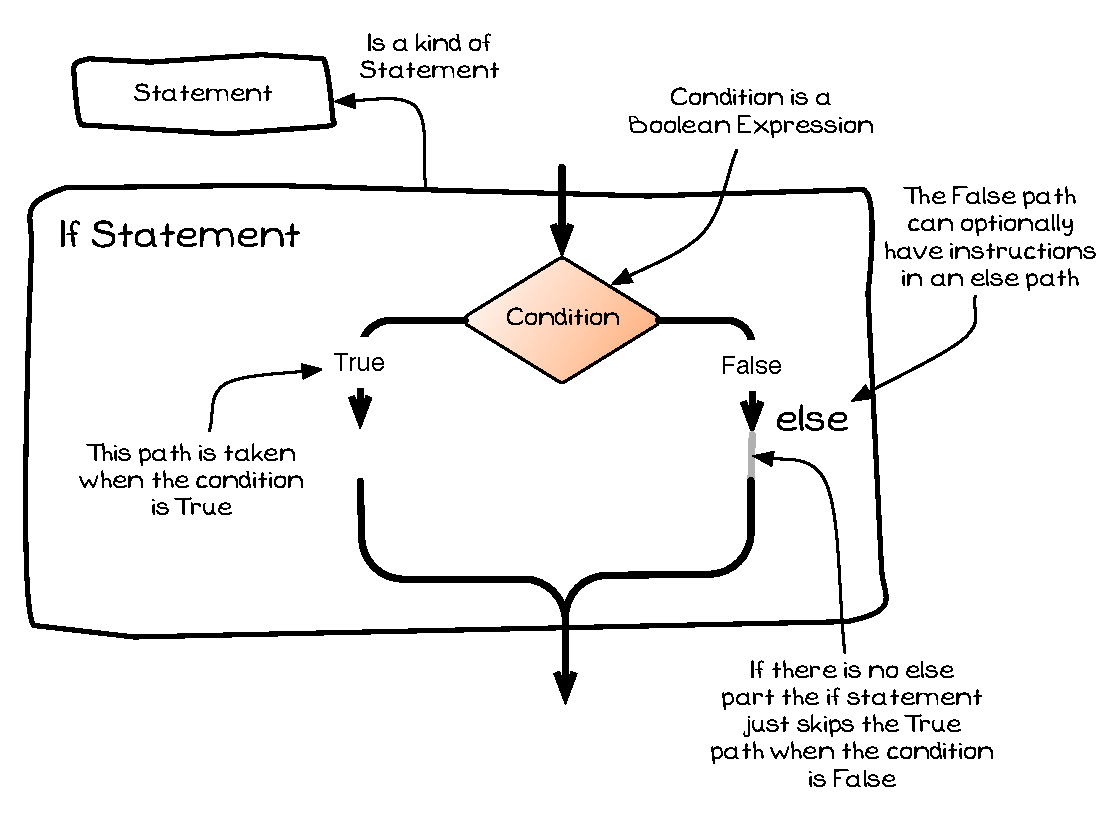
\includegraphics[width=\textwidth]{./topics/control-flow/diagrams/IfStatement} 
   \caption{If statement lets you selectively run a branch of code}
   \label{fig:branching-if-statement}
\end{figure}

\mynote{
\begin{itemize}
  \item An if statement is an \textbf{action}. It allows you to command the computer to select a path based on a Boolean expression.
  \item The if statement has two branches, one that is taken when the condition is True, the other when it is False.
  \item The False branch may \emph{optionally} have instructions that are carried out when the condition is False. 
  \item If there are no instructions you want performed when the condition is False you do not need to include an else branch, and the if statement will just skip the True branch when the condition is False.
  \item The if statement has one entry point, two paths, and then one exit point.
\end{itemize}
}


% subsection if_statement (end)
\clearpage
\subsection{Boolean Data} % (fold)
\label{sub:boolean_data}

The Boolean\footnote{Named after George Bool's Boolean logic.} Data Type is a \nameref{sub:type} used to represent \textbf{truth}. A Boolean value will either be \textbf{true} or \textbf{false}. These values are used extensively in the control flow statements to determine the action to perform.

\begin{figure}[h]
   \centering
   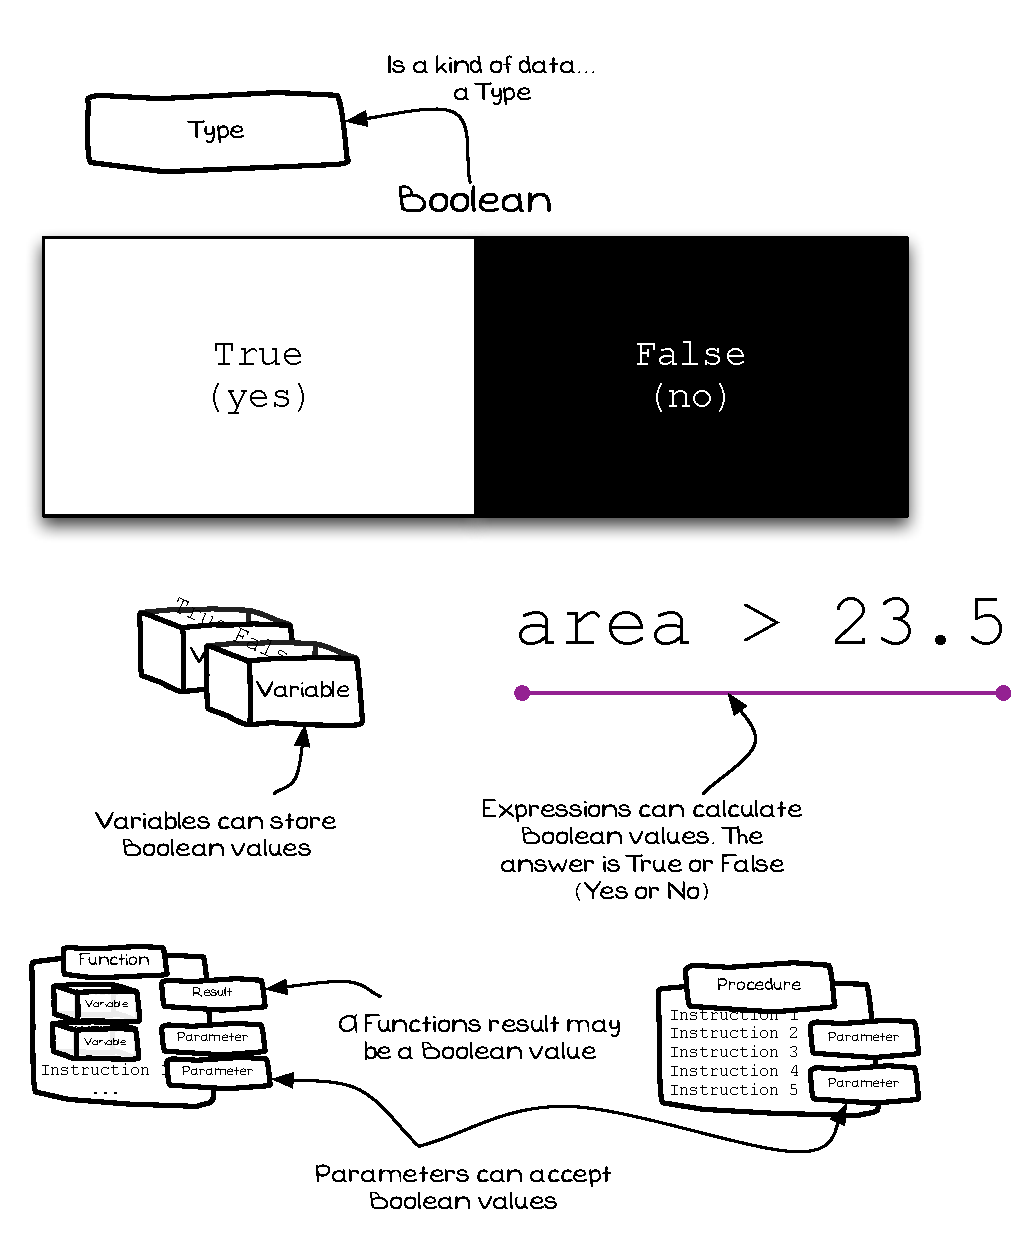
\includegraphics[width=0.8\textwidth]{./topics/control-flow/diagrams/BooleanData} 
   \caption{Boolean data represents truth}
   \label{fig:boolean-data}
\end{figure}

\mynote{
\begin{itemize}
  \item Boolean is an existing \textbf{artefact}, it is a \nameref{sub:type} that has been defined to represent truth values.
  \item A Boolean value is either \textbf{true} or \textbf{false}. You can also think of these as \emph{yes} and \emph{no}.
  \item Boolean values are used in most of the control flow statements.
  \item The Boolean type can be used in the same way as other types.
\end{itemize}
}
% subsection boolean_data (end)

\clearpage
\subsubsection{Comparisons} % (fold)
\label{sub:comparisons}

Comparisons are a common way of getting Boolean values in your code. These \nameref{sub:expression}s allow you to compare two values to check for a given condition. For example, the Expression shown in Figure \ref{fig:boolean-data} is asking if the \emph{value} in the \texttt{area} variable is larger than \texttt{23.5}. The result of this expression will be either \texttt{true} or \texttt{false} depending on the current value stored in \texttt{area}. Table \ref{tbl:bool-expr-sample} lists some example values for this expression, given different values stored in the \texttt{area} variable.

\begin{table}[h]
  \centering
  \begin{tabular}{|c|c|}
    \hline
    \textbf{Value in \texttt{area}} & \textbf{\texttt{area > 23.5}} \\
    \hline
    \texttt{73.2} & \texttt{true} \\
    \hline
    \texttt{-2.5} & \texttt{false} \\
    \hline
    \texttt{23.5} & \texttt{false} \\
    \hline
  \end{tabular}
  \caption{Example values for the expression \texttt{area > 23.5}}
  \label{tbl:bool-expr-sample}
\end{table}

Programming languages offer a range of different comparison operators. These typically include comparisons to check if values are the same or different, and to check if one value is larger or small than another. The different operators for C and Pascal are listed in Table \ref{tbl:comparisons}.

\begin{table}[h]
  \centering
  \begin{tabular}{|c|c|c|c|}
    \hline
     & \textbf{Description} & \textbf{C} & \textbf{Pascal} \\
    \hline
    \textbf{Equal} & Are the values the same? & \texttt{a == b} & \texttt{a = b} \\
    \hline
    \textbf{Not Equal} & Are the values different? & \texttt{a != b} & \texttt{a <> b} \\
    \hline
    \textbf{Larger Than} & Is the left value larger than the right? & \multicolumn{2}{c|}{\texttt{a > b}}  \\
    \hline
    \textbf{Less Than} & Is the left value smaller than the right? & \multicolumn{2}{c|}{\texttt{a < b}}  \\
    \hline
    \textbf{Larger Or Equal} & Is the left value equal or larger than the right? & \multicolumn{2}{c|}{\texttt{a >= b}}  \\
    \hline
    \textbf{Less Or Equal} & Is the left value smaller or equal to the right? & \multicolumn{2}{c|}{\texttt{a <= b}}  \\
    \hline
    
  \end{tabular}
  \caption{Comparison Operators}
  \label{tbl:comparisons}
\end{table}

\mynote{
\begin{itemize}
  \item Comparisons can only be performed between \textbf{two} values.
  \item The values on either side of the comparison are \nameref{sub:expression}s, allowing you to calculate the values being compared.
\end{itemize}
}

\csection{
C uses a double equal (\texttt{==}) for comparison as the single equals (\texttt{=}) is used for assignment.
}

% subsection comparisons (end)

\clearpage
\subsubsection{Logical Operators} % (fold)
\label{sub:logical_operators}

The comparison operators allow you to compare \emph{two} values. This is very useful, but in itself is incomplete. What, for example, do you do when you want to compare three or more values? While you are limited to two values with the comparison operators, there are other operators that allow you to \textbf{combine} Boolean expressions. This will enable you to combine together multiple Boolean values into a single Expression.

There are four main \emph{logical operators}: \textbf{and}, \textbf{or}, \textbf{xor}, and \textbf{not}. Each of these operators works on two Boolean values, combining them to give a new Boolean value. For example, the \emph{and} operator allows you to check if \emph{both} of the expressions are true. The expression \texttt{area > 0 and area < 10} will be true only when area is both larger than zero and less then ten.

\begin{figure}[h]
   \centering
   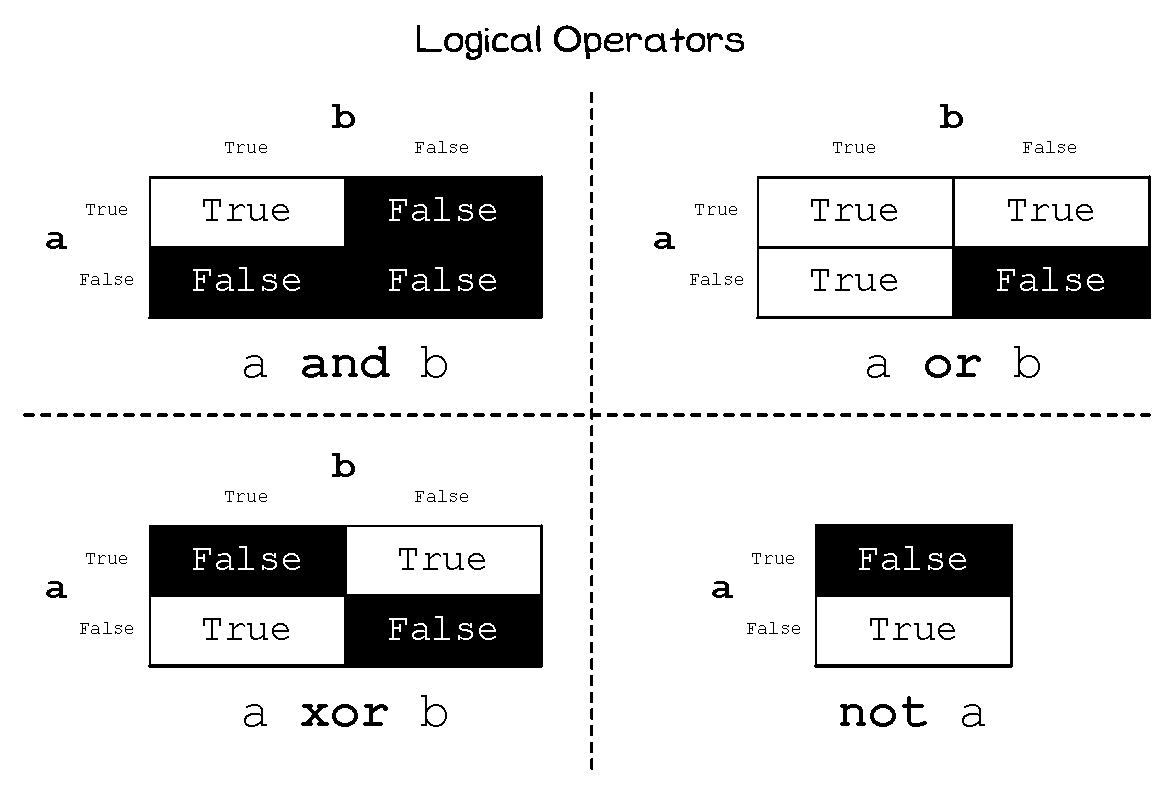
\includegraphics[width=0.7\textwidth]{./topics/control-flow/diagrams/LogicalOperators} 
   \caption{Logical Operators combine Boolean values}
   \label{fig:logical-operators}
\end{figure}

\begin{table}[h]
  \centering
  \begin{tabular}{|c|c|c|c|}
    \hline
     & \textbf{Description} & \textbf{C} & \textbf{Pascal} \\
    \hline
    \textbf{And} & Are both values True? & \texttt{a \&\& b} & \texttt{a and b} \\
    \hline
    \textbf{Or} & Is at least one value True? & \texttt{a || b} & \texttt{a or b} \\
    \hline
    \textbf{Xor} & Is one value True, and the other False? & \texttt{a \^{} b} & \texttt{a xor b} \\
    \hline
    \textbf{Not} & Is the value False? & \texttt{!a} & \texttt{not a}  \\
    \hline
  \end{tabular}
  \caption{Logical Operators}
  \label{tbl:logical-operators}
\end{table}

\begin{table}[h]
  \centering
  \begin{tabular}{|c|c|c|c|c|c|}
    \hline
    \multirow{2}{*}{area }& \multirow{2}{*}{\texttt{area > 0}} & \multirow{2}{*}{\texttt{area < 10}} & \multicolumn{3}{c|}{\texttt{area > 0 {\textbf{\ldots}} area < 10}} \\
    \cline{4-6}
     &  &  & \textbf{and} & \textbf{or} & \textbf{xor} \\
    \hline
    \texttt{\textbf{5}} & True & True & True & True & False \\
    \hline
    \texttt{\textbf{27}} & True & False & False & True & True \\
    \hline
    \texttt{\textbf{0}} & False & True & False & True & True \\
    \hline
  \end{tabular}
  \caption{Example Logical Expressions}
  \label{tbl:example_logical_expr}
\end{table}

\mynote{
\begin{itemize}
  \item Table \ref{tbl:example_logical_expr} has some example expressions.
  \item The tables in Figure \ref{fig:logical-operators} show the values of the different logical operators. These are known as \textbf{Truth Tables}.
  \item Table \ref{tbl:logical-operators} outlines the different logical operators, and how they are coded in C and Pascal.
\end{itemize}
}



% subsection boolean_logic (end)
\clearpage
\subsubsection{Case Statement} % (fold)
\label{sub:case_statement}

The case statement is the second kind of branching statement. This allows you to create paths that execute based on matching a value from an expression. This allows one case statement to handle many alternative paths.

\begin{figure}[h]
   \centering
   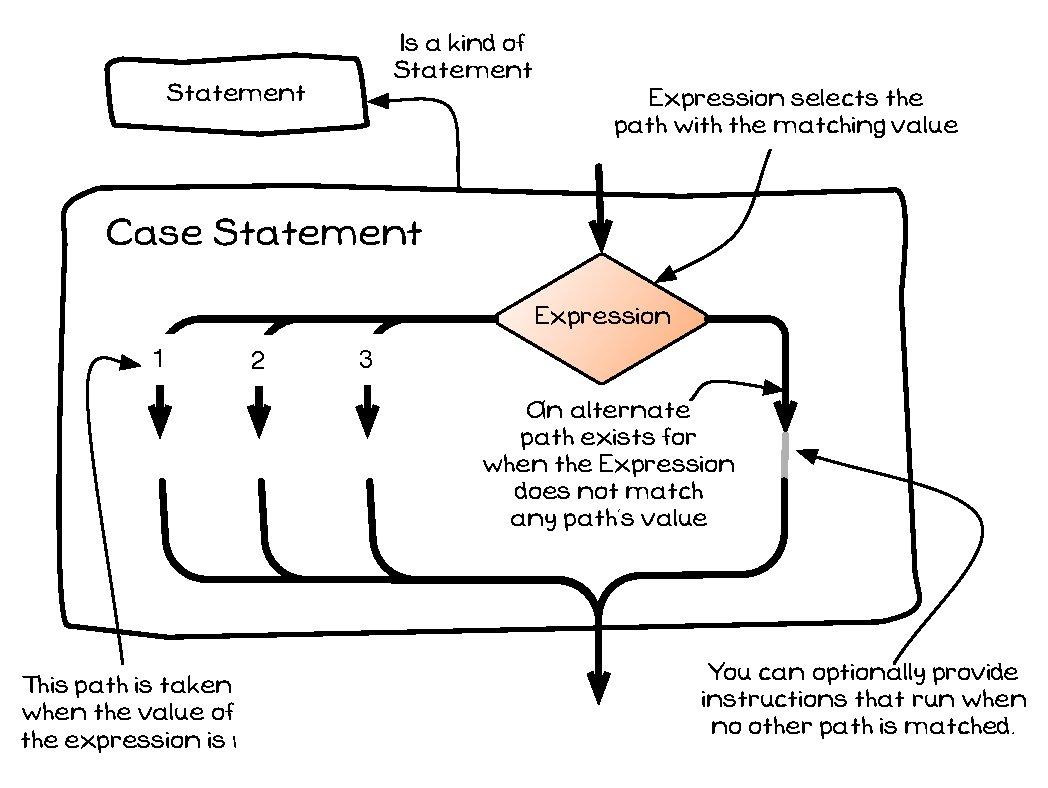
\includegraphics[width=\textwidth]{./topics/control-flow/diagrams/CaseStatement} 
   \caption{Case statement selectively runs multiple branches of code}
   \label{fig:branching-case-statement}
\end{figure}

\mynote{
\begin{itemize}
  \item The case statement is a kind of \textbf{action}. It allows you to command the computer to select a path based upon the value of an expression.
  \item Each path within the Case Statement has a value. When the computer executes the case statement the path values are used to determine which path will be taken.
  \item In C and Pascal the Case Statement only works with Ordinal Values. This limits you to using Character or Integer values within the Case Statement's Expression.
  \item The Case Statement has one entry point, multiple paths, and then one exit point.
\end{itemize}
}

% section case_statement (end)
\clearpage
\subsection{Compound Statement} % (fold)
\label{sub:compound_statement}

\nameref{sub:branching} and \nameref{sub:looping} statements need to be able to include a number of instructions within their paths. Often languages will manage this by indicating that only a \emph{single} statement can be included in any of these paths, and then include the ability to code multiple statements in a \emph{single compound statement}.

\begin{figure}[h]
   \centering
   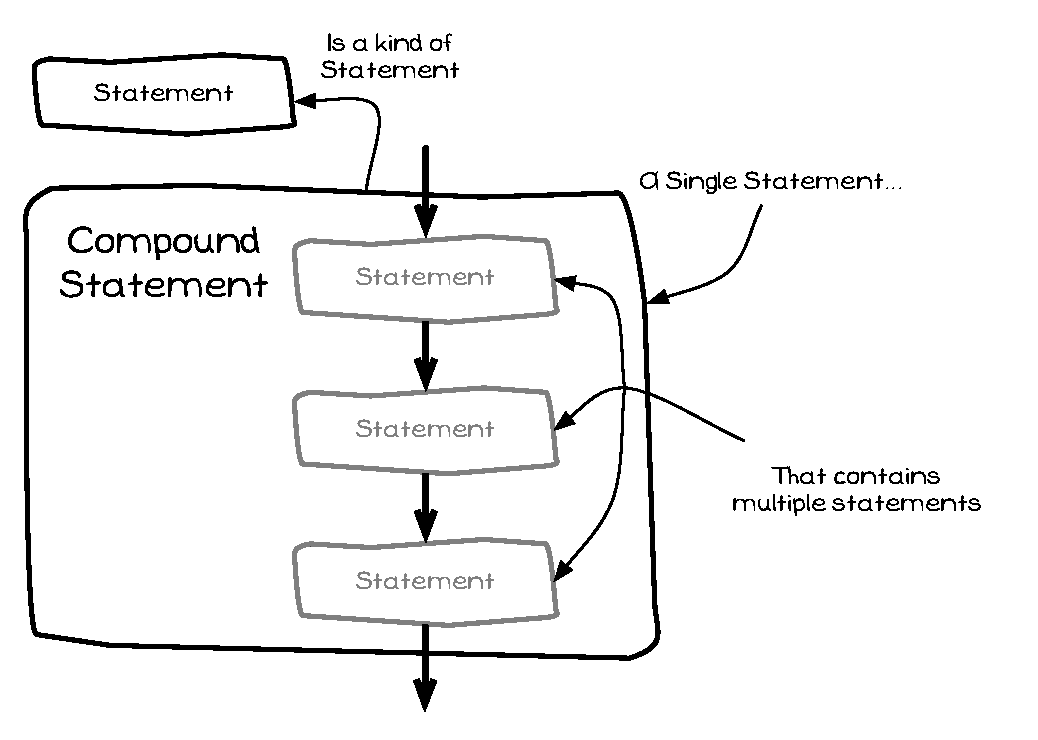
\includegraphics[width=\textwidth]{./topics/control-flow/diagrams/CompoundStatement} 
   \caption{A Compound Statement is a Statement that can contain other Statements}
   \label{fig:branching-compound-statement}
\end{figure}

\mynote{
\begin{itemize}
  \item A Compound Statement is a way of grouping \textbf{action}s, allowing you to create a single statement that contains multiple statements.
  \item Compound Statements are useful when combined with \nameref{sub:branching} and \nameref{sub:looping} Statements. Allowing you to put multiple statements within a path.
\end{itemize}
}

% subsection compound_statements (end)
\clearpage
\subsection{Statement (with Branches)} % (fold)
\label{sub:statement_with_branches_}

\begin{figure}[h]
   \centering
   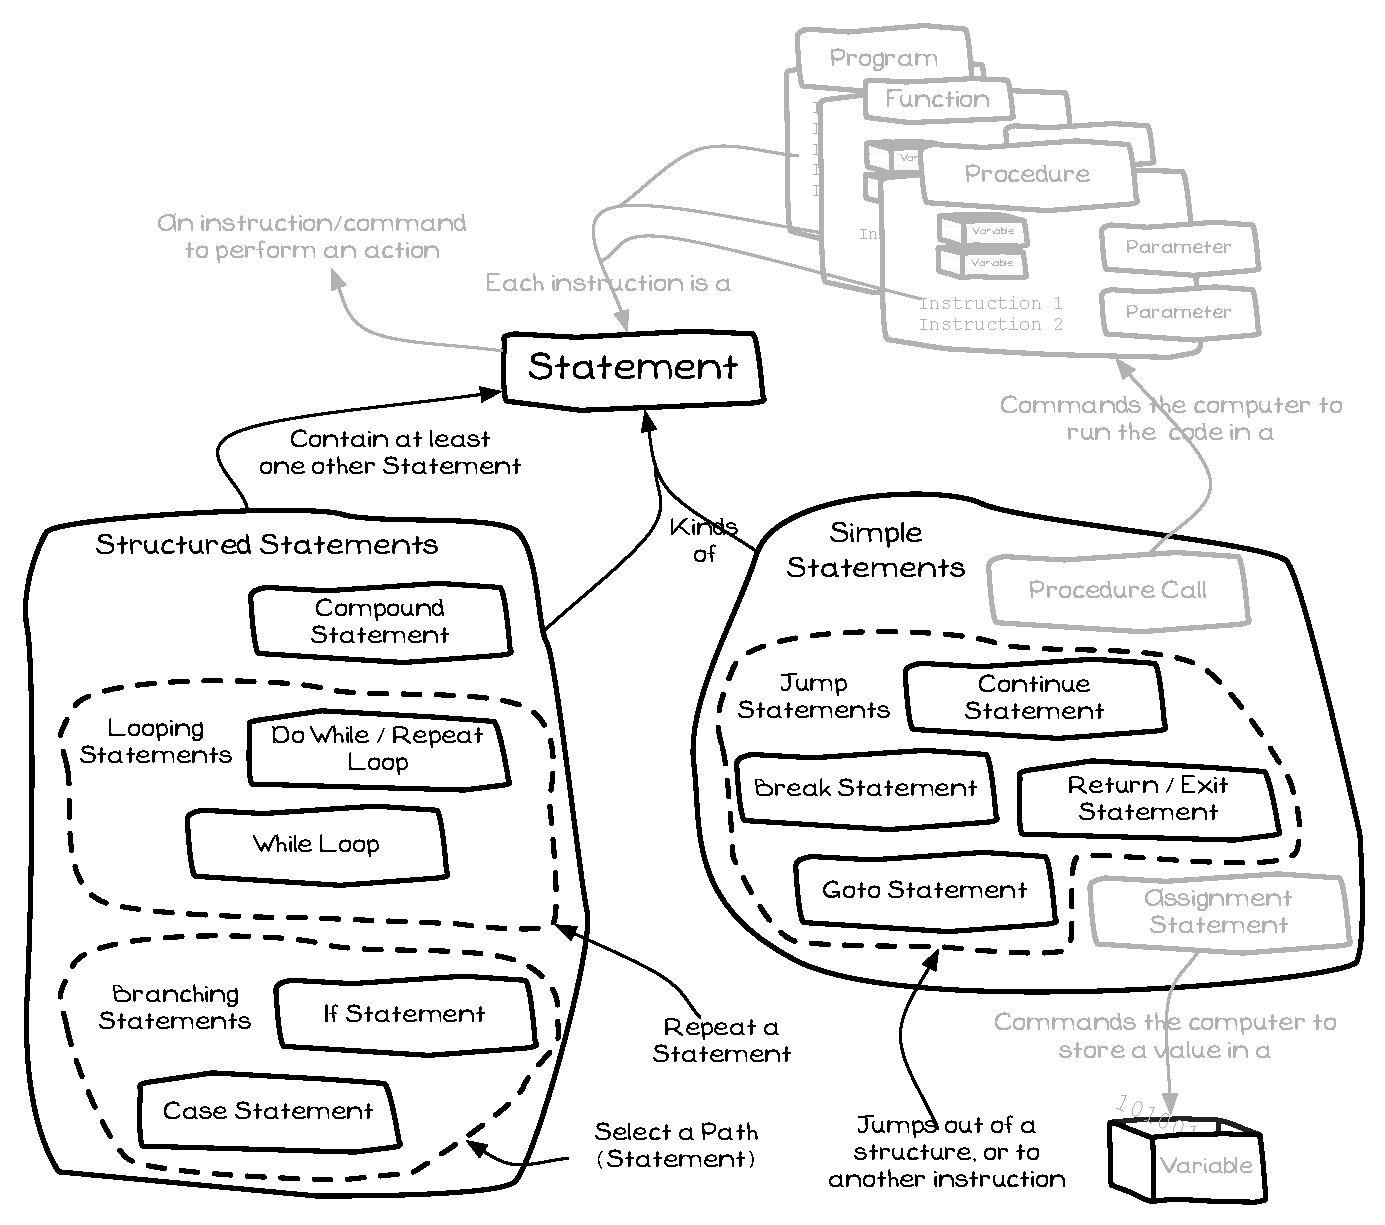
\includegraphics[width=\textwidth]{./topics/control-flow/diagrams/Statement} 
   \caption{A Statement may be a Branching Statement: an If or Case Statement}
   \label{fig:branching-statement}
\end{figure}


% subsection statement_with_branches_ (end)

% section branching_concepts (end)


% =============
% = C Section =
% =============
\clearpage
\section{Branching in C} % (fold)
\label{sec:branching_in_c}

\clearpage
\subsection{C Statement (with Branches)} % (fold)
\label{sub:c_statement_with_branches_}

\csyntax{csynt:branching-statement-with-branches}{a Statement (with branches)}{branching/statement-with-branches}

% subsection c_statement_with_branches_ (end)
\clearpage
\subsection{C If Statement} % (fold)
\label{sub:c_if_statement}

The if statement is a \nameref{sub:branching} statement. This can be used to optionally run a block of code, providing two alternate paths controlled by a Boolean expression.

\csyntax{csynt:branching-if-statement}{an If Statement}{branching/if-statement}

\csection{\ccode{clst-test-if}{C if test code}{code/c/control-flow/test-if.c}}

\mynote{
\begin{itemize}
  \item This is the C syntax for the \nameref{sub:if_statement}.
  \item The parenthesis surround the expression. This enables the compiler to tell where the expression ends.
  \item Notice that the \texttt{else} branch is optional.
  \item When the expression is \texttt{false} (0 in C), the else branch is taken.
  \item For any other value the first path is taken.
  \item You only need to include \texttt{stdbool.h} if you want to use the \texttt{bool} type and the values \texttt{true} or \texttt{false}.
\end{itemize}
}

% subsection c_if_statement (end)
\clearpage
\subsection{C Case Statement} % (fold)
\label{sub:c_case_statement}

The case statement allows you to switch between a number of paths.

\csyntax{csynt:branching-case-statement}{a Case Statement}{branching/case-statement}

\mynote{
\begin{itemize}
  \item This is the C syntax to declare a \nameref{sub:case_statement}.
  \item The \emph{constant expressions} in each \emph{case} must be ordinal values (integers or characters).
  \item The code in \lref{clst-test-case} shows an example use for a case statement.
  \item The \texttt{default} path is taken when none of the other paths match the expression.
  \item If the \texttt{break} is left off the end of a \emph{case} then execution will continue into the next \emph{case}. For example, in \lref{clst-simple-case} if the user enters `c' the output will be `\texttt{C and D}'
  \item Each \emph{case} can contain a number of Statements.
  \item Watch \url{http://www.youtube.com/watch?v=zIV4poUZAQo} for important details on the legendary Knights of Ni.
\end{itemize}
}

\csection{\ccode{clst-simple-case}{C case test code with a character}{code/c/control-flow/simple-case.c}}

\clearpage

\csection{\ccode{clst-test-case}{C case test code with an integer}{code/c/control-flow/test-case.c}}

% subsection case_statement (end)
\clearpage
\subsection{C Compound Statement} % (fold)
\label{sub:c_compound_statement}

Most of the C structured statements only allow single statements within each path. For example, the paths in the two branches of an \nameref{sub:c_if_statement} can only contain a single statement. The \nameref{sub:compound_statement} allows you to group together multiple statements within a single \emph{compound statement}.

\csyntax{csynt:branching-compound-statement}{a Compound Statement}{branching/compound-statement}

\csection{\ccode{clst-test-compound}{C compound statement test code}{code/c/control-flow/test-compound.c}}

\mynote{
\begin{itemize}
  \item \fref{csynt:branching-compound-statement} shows the syntax for a \nameref{sub:compound_statement} in C.
  \item The code in \lref{clst-test-compound} shows an if statement that includes two compound statements within its branches.
  \item Compound statements in C are marked with curly brackets, `\{' for the start, and `\}' for the end.
  \item The compound statement is a standard statement, and can be used anywhere a statement can appear. Its practice use is for grouping statements within other structured statements, and you are unlikely to find it used in any other way.
\end{itemize}
}

% subsection c_compound_statement (end)
\clearpage
\subsection{C Boolean Data} % (fold)
\label{sub:c_boolean_data}

C has very flexible support for Boolean values. In C a \texttt{0} value is considered to be false, and any other value is true. Modern C compilers have now added support for an explicit Boolean type, \texttt{bool}. This type requires the \texttt{stdbool.h} header file, which defines the \texttt{bool} type as well as the values \texttt{true} and \texttt{false}.

\begin{table}[h] 
\begin{minipage}{\textwidth}
\centering
\begin{tabular}{|l|c|c|}
\hline
\multicolumn{3}{|c|}{\textbf{Boolean Type}} \\
\hline
\emph{Name} & \emph{Size} & \emph{Values} \\
\hline
\texttt{bool} & 1 byte/8 bits & \texttt{true} or \texttt{false} \\
\hline
\end{tabular}
\caption{C Boolean Type}\label{tbl:c-boolean}
\end{minipage}
\end{table}

\begin{table}[h]
  \centering
  \begin{tabular}{|c|c|c|}
    \hline
     & \textbf{Description} & \textbf{C} \\
    \hline
    \textbf{Equal} & Are the values the same? & \texttt{a == b} \\
    \hline
    \textbf{Not Equal} & Are the values different? & \texttt{a != b} \\
    \hline
    \textbf{Larger Than} & Is the left value larger than the right? & \texttt{a > b}  \\
    \hline
    \textbf{Less Than} & Is the left value smaller than the right? & \texttt{a < b}  \\
    \hline
    \textbf{Larger Or Equal} & Is the left value equal or larger than the right? & \texttt{a >= b}  \\
    \hline
    \textbf{Less Or Equal} & Is the left value smaller or equal to the right? & \texttt{a <= b}  \\
    \hline
  \end{tabular}
  \caption{C Comparison Operators}
  \label{tbl:c_comparison_op}
\end{table}

\begin{table}[h]
  \centering
  \begin{tabular}{|c|c|c|}
    \hline
     & \textbf{Description} & \textbf{C} \\
    \hline
    \textbf{And} & Are both values True? & \texttt{a \&\& b} \\
    \hline
    \textbf{Or} & Is at least one value True? & \texttt{a || b} \\
    \hline
    \textbf{Xor} & Is one value True, and the other False? & \texttt{a \^{} b} \\
    \hline
    \textbf{Not} & Is the value False? & \texttt{!a} \\
    \hline
  \end{tabular}
  \caption{Logical Operators}
  \label{tbl:c-logical-operators}
\end{table}

\mynote{
\begin{itemize}
  \item To use the Boolean type in C you must include the \texttt{stdbool.h} header.
  \item In C false is the value \texttt{0}, and true is any other value.
  \item The \texttt{stdbool.h} header gives you access to two value, \texttt{true} and \texttt{false}. \texttt{true} has the value 1, \texttt{false} has the value 0.
\end{itemize}
}

\clearpage

\csection{\ccode{clst:bool-test}{C Boolean Test Code}{code/c/control-flow/test-bools.c}}


% subsection c_boolean_data (end)


% section branching_in_c (end)


% chapter branching (end)